\chapter{Between-firm growth correlations}
\label{app:correlations}

The granular models fail, \citet{moran2024} argue, because they lack a correlation between the
growth rates of different firms, and they conjecture that this correlation grows with firm size:
the missing ingredient is that ``the correlation of a firm's growth rate with that of the whole
economy and the correlation of the growth rate of firms of similar sizes clearly grow with their
size''. The body of this thesis reproduces the size-conditioned statistics through the degree
heterogeneity of the interaction graph. That leaves a direct question, which this appendix
settles: does the model reproduce the empirical facts by the route \citet{moran2024} conjecture,
through correlations that grow with size, or by another?

We measure two correlations from the per-firm growth time series $g_i(t) = \Delta \ln S_i$ in the
fluctuating state, on the thesis graph (power-law $2.5$, mean degree $C = N/40$, $N = 16000$, ten
economies). The first is the co-movement of a firm with the aggregate,
$\rho_i = \mathrm{corr}_t\!\big(g_i(t),\,\bar g(t)\big)$, where $\bar g(t)$ is the
cross-sectional mean growth: it measures how strongly a firm tracks the common motion of the
economy. The second is the mean pairwise correlation
$\mathrm{corr}_t\!\big(g_i(t),\,g_j(t)\big)$ among firms that fall in the same bin, the direct
analogue of \citet{moran2024}'s ``correlation of firms of similar sizes''. Each is binned both by
firm size and by degree.

Both correlations are small and, to the precision reached here, flat
(Figure~\ref{fig:correlations}). The co-movement with the aggregate sits at $\rho \approx 0.09$
and is independent of size and of degree across the ranges resolved. The same-bin pairwise
correlation is an order of magnitude smaller, $\approx 0.01$, also flat, with at most a weak rise
to $\approx 0.018$ among the very largest firms. The correlations \citet{moran2024} name are thus
present but modest, and they do not grow appreciably with either size or degree.

The model therefore reproduces the size-conditioned anomalies \emph{without} the size-growing
correlations \citet{moran2024} conjecture. Its mechanism is instead the degree-dependence of the
noise \emph{amplitude}: under the dilute normalization a firm's own idiosyncratic noise variance
grows with its connectivity (Section~\ref{sec:growing-graph}), a single-firm property, riding on a
flat and modest between-firm correlation background. The model is in this sense an alternative to
\citet{moran2024}'s hypothesis rather than a realization of it: the anomalies need not come from
correlations that strengthen with size.

Two limits qualify the null result. The pairwise measure averages over same-bin pairs that are
almost all unconnected on the sparse graph, so it understates the correlation between direct
trading partners, which a production-network reading of the model would emphasize. And the
survival mechanism of Section~\ref{sec:growing-degree-size} removes the extreme hubs from the
fluctuating state: the live-firm degree axis reaches only $k \approx 470$ although the graph's
tail extends beyond $k \approx 3000$, so the most connected firms, where any correlation would be
strongest, are absent from the measurement. A direct test on firm-level data with a known
interaction network, where both restrictions could be lifted, remains open.

\begin{figure}[htbp]
    \centering
    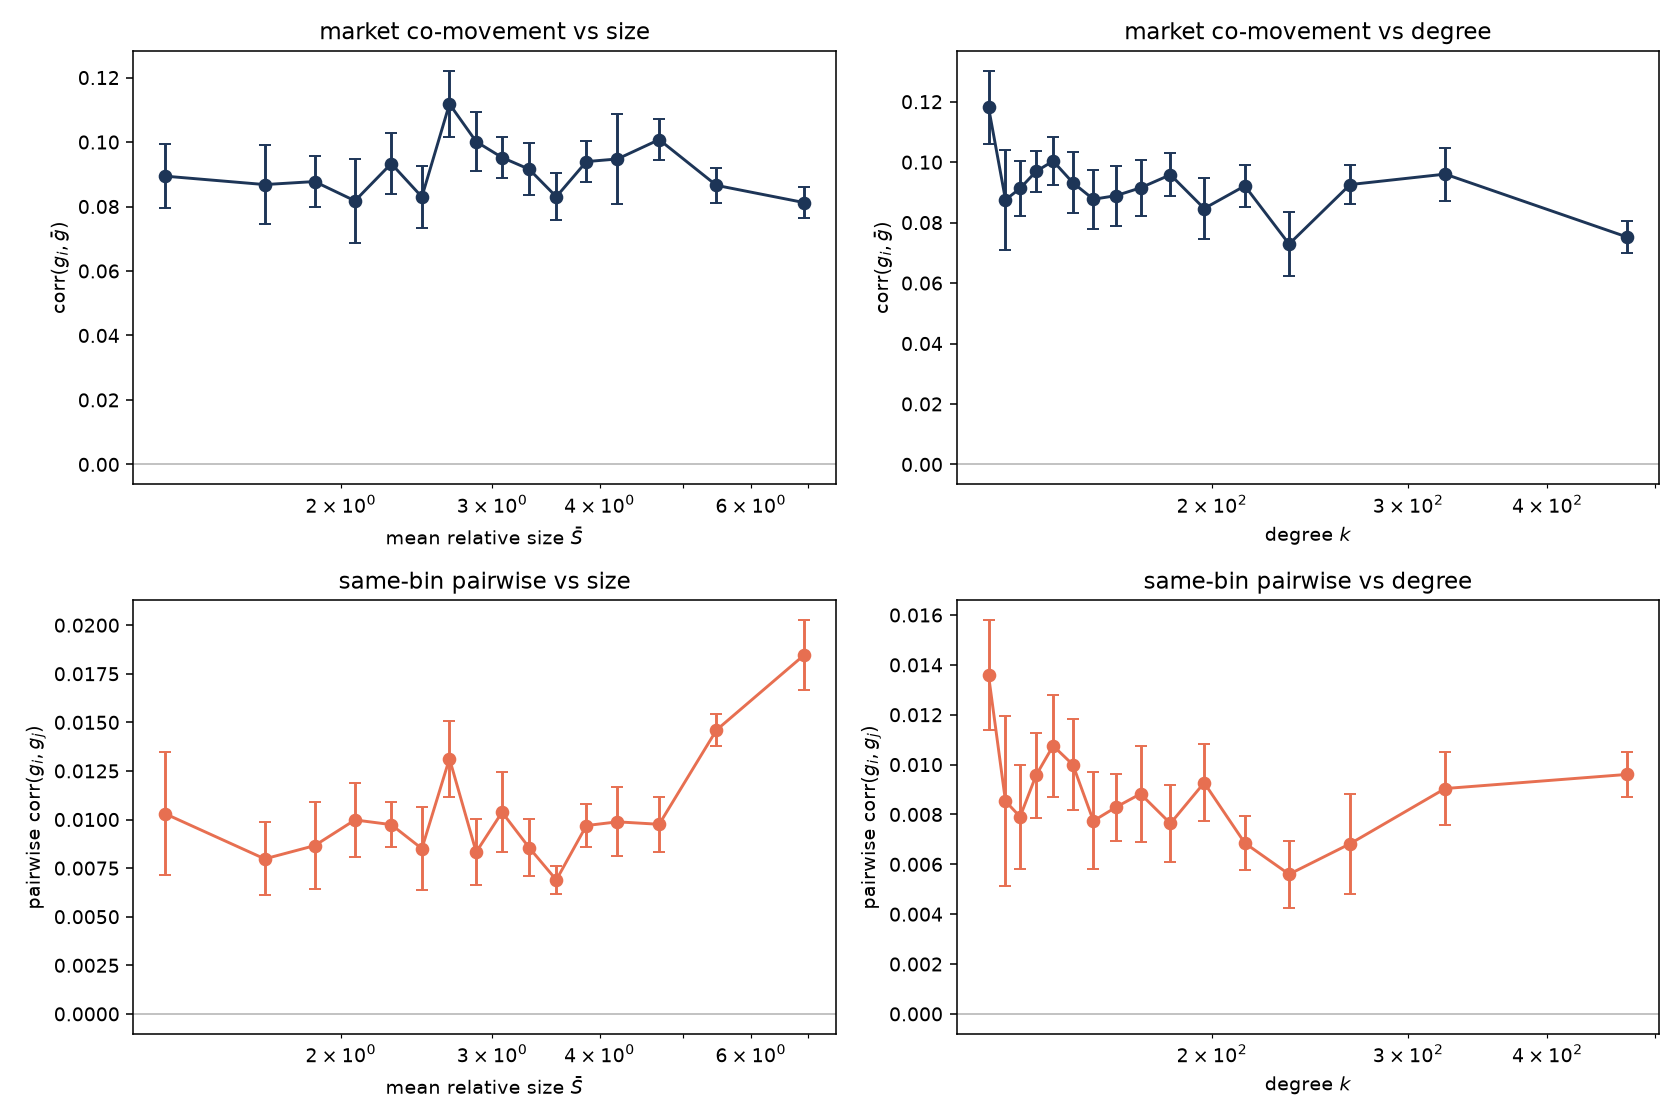
\includegraphics[width=\linewidth]{between_firm_corr.png}
    \caption{Between-firm growth correlations in the fluctuating state
    ($N = 16000$, ten economies, power-law-$2.5$ graph). \panel{Top}: the co-movement of each
    firm with the aggregate, $\mathrm{corr}(g_i, \bar g)$, against firm size (left) and degree
    (right); flat at $\approx 0.09$ on both axes. \panel{Bottom}: the mean pairwise correlation
    among firms in a bin, against size (left) and degree (right); flat at $\approx 0.01$, with a
    weak rise among the largest firms. Neither correlation grows appreciably with size or degree,
    so the model reproduces the size-conditioned statistics through the degree-dependent noise
    amplitude rather than through the size-growing correlations of \citet{moran2024}.}
    \label{fig:correlations}
\end{figure}
